\chapter{Solution Design}

\section{Algorithm Description}

The algorithm implemented for the ray tracer, which is the one described in \cite{thorne15}, assumes the following:
\begin{enumerate}
	\item The universe is modelled by the Kerr metric written in Boyer-Lindquist coordinates (see \autoref{eq:kerrmetric}), with a black hole in the centre of the spatial coordinates parametrized by its spin $a$. Its mass is assumed to be 1.
	\item We define a family of observers (FIDO) at rest in space with orthonormal basis vectors $\{e_{\widehat{r}}, e_{\widehat{\vartheta}}, e_{\widehat{\varphi}}\}$, pointing along the spatial coordinate lines.
	\item A camera is placed outside of the horizon of the black hole.
	\begin{enumerate}
		\item The position of the camera is described by the coordinates $\{r_c, \vartheta_c, \varphi_c\}$.
		\item The camera speed with respect to the FIDO is noted as $\beta$.
		\item The direction of motion relative to the FIDO is described by a unit vector $B$ in the camera's reference frame.
		\item We set up a right-handed coordinate system placed on the camera's reference frame, with orthonormal basis $\{e_x, e_y, e_z\}$, where
		\begin{itemize}
			\item $e_y$ is identified with $B$, \ie, it points to the direction of motion of the camera.
			\item $e_x$ is perpendicular to $e_y$ and contained on the plane $\langle e_{\widehat{r}}, e_{\widehat{\vartheta}} \rangle$.
			\item $e_z$ is perpendicular to $e_x$ and to $e_y$.
		\end{itemize}
		\item We set up a spherical coordinate system derived from the previous one, noted as $\{\vartheta_{cs}, \varphi_{cs}\}$, where:
		\begin{itemize}
			\item $\vartheta$ is the polar angle with respect to the coordinate system origin.
			\item $\varphi$ is the azimuthal angle with respect to the coordinate system origin. The black hole is assumed to rotate in the positive $\varphi$ direction.
		\end{itemize}
	\end{enumerate}
\end{enumerate}

The algorithm consider a set of timelike geodesics arriving at the camera. These geodesics are then integrated backwards to obtain the ray's point of origin on the celestial sphere (at $r = \infty$). These points are noted as $(\vartheta', \varphi')$.

In short, the algorithm goal is to compute the following map
\begin{equation}
	\label{eq:initmap}
	(\vartheta_{cs}, \varphi_{cs}) \xmapsto{\mathfrak{h}_1} (\vartheta', \varphi')
\end{equation}
for each considered geodesic arriving at the camera.

One could take this algorithm description and, using the equations on \autoref{theo:eqsmotion}, integrate geodesics whose final point is an arbitrary $(\vartheta_{cs}, \varphi_{cs})$.

This work, however, aims to generate realistic images of what an observer would see when looking at a black hole from near distances. With this goal in mind, the camera is abstracted as a simple, yet effective, model that will let us produce such images.

\subsection{Pinhole Camera}

The camera considered in the work follows the \emph{pinhole camera model}, which assumes a camera with an infinitely small diaphragm that focuses all the incoming rays onto its sensor.

The camera is described by the following parameters:
\begin{enumerate}
	\item The position on the Kerr spacetime, described by the spatial Boyer-Lindquist coordinates $\{r_c, \vartheta_c, \varphi_c\}$.
	\item The \emph{sensor} (that can be though as the film or the CCD of a usual camera), which is described by its \emph{resolution} (number of pixels per column and number of pixels per row) and by its size (width and height in physical units).
	\item The \emph{focal point}, $F$: a point in the line perpendicular to the sensor and going through its centre. This point will collect all incoming rays and can be though as the diaphragm, whose aperture is infinitely small.
	\item The \emph{focal distance}, $d$: distance from the focal point to the sensor.
	\item The \emph{pitch}, \emph{roll} and \emph{yaw} angles, that describe the rotation of the sensor on each of its axis, depicted in figure \fixme{add figure}.
\end{enumerate}

This model let us compute the direction of the incoming rays just by indexing the particular pixel they hit, obtaining a map
\begin{equation}
	\label{eq:pixelmap}
	(p_x, p_y) \xmapsto{\mathfrak{h}_2} (\vartheta_{cs}, \varphi_{cs}),
\end{equation}
where $(p_x, p_y)$ are the components of the pixel in a system of coordinates whose origin is placed at the top-left corner of the sensor.

By composing \autoref{eq:initmap} and \autoref{eq:pixelmap}, we define the map
\begin{equation}
	(p_x, p_y) \xmapsto{\mathfrak{h} = \mathfrak{h_1}\circ\mathfrak{h_2}} (\vartheta', \varphi'),
\end{equation}
that summarises all the work the algorithm does: from a pixel on the camera's reference frame, we compute the origin of the incoming ray that hit that pixel.

\subsection{Pixel to Ray Map}

Let us consider a pixel $P$ whose coordinates on the sensor's reference frame are $(p_x, p_y)$, as depicted in \autoref{fig:pinhole}.

\begin{figure}[bth]
	\myfloatalign
	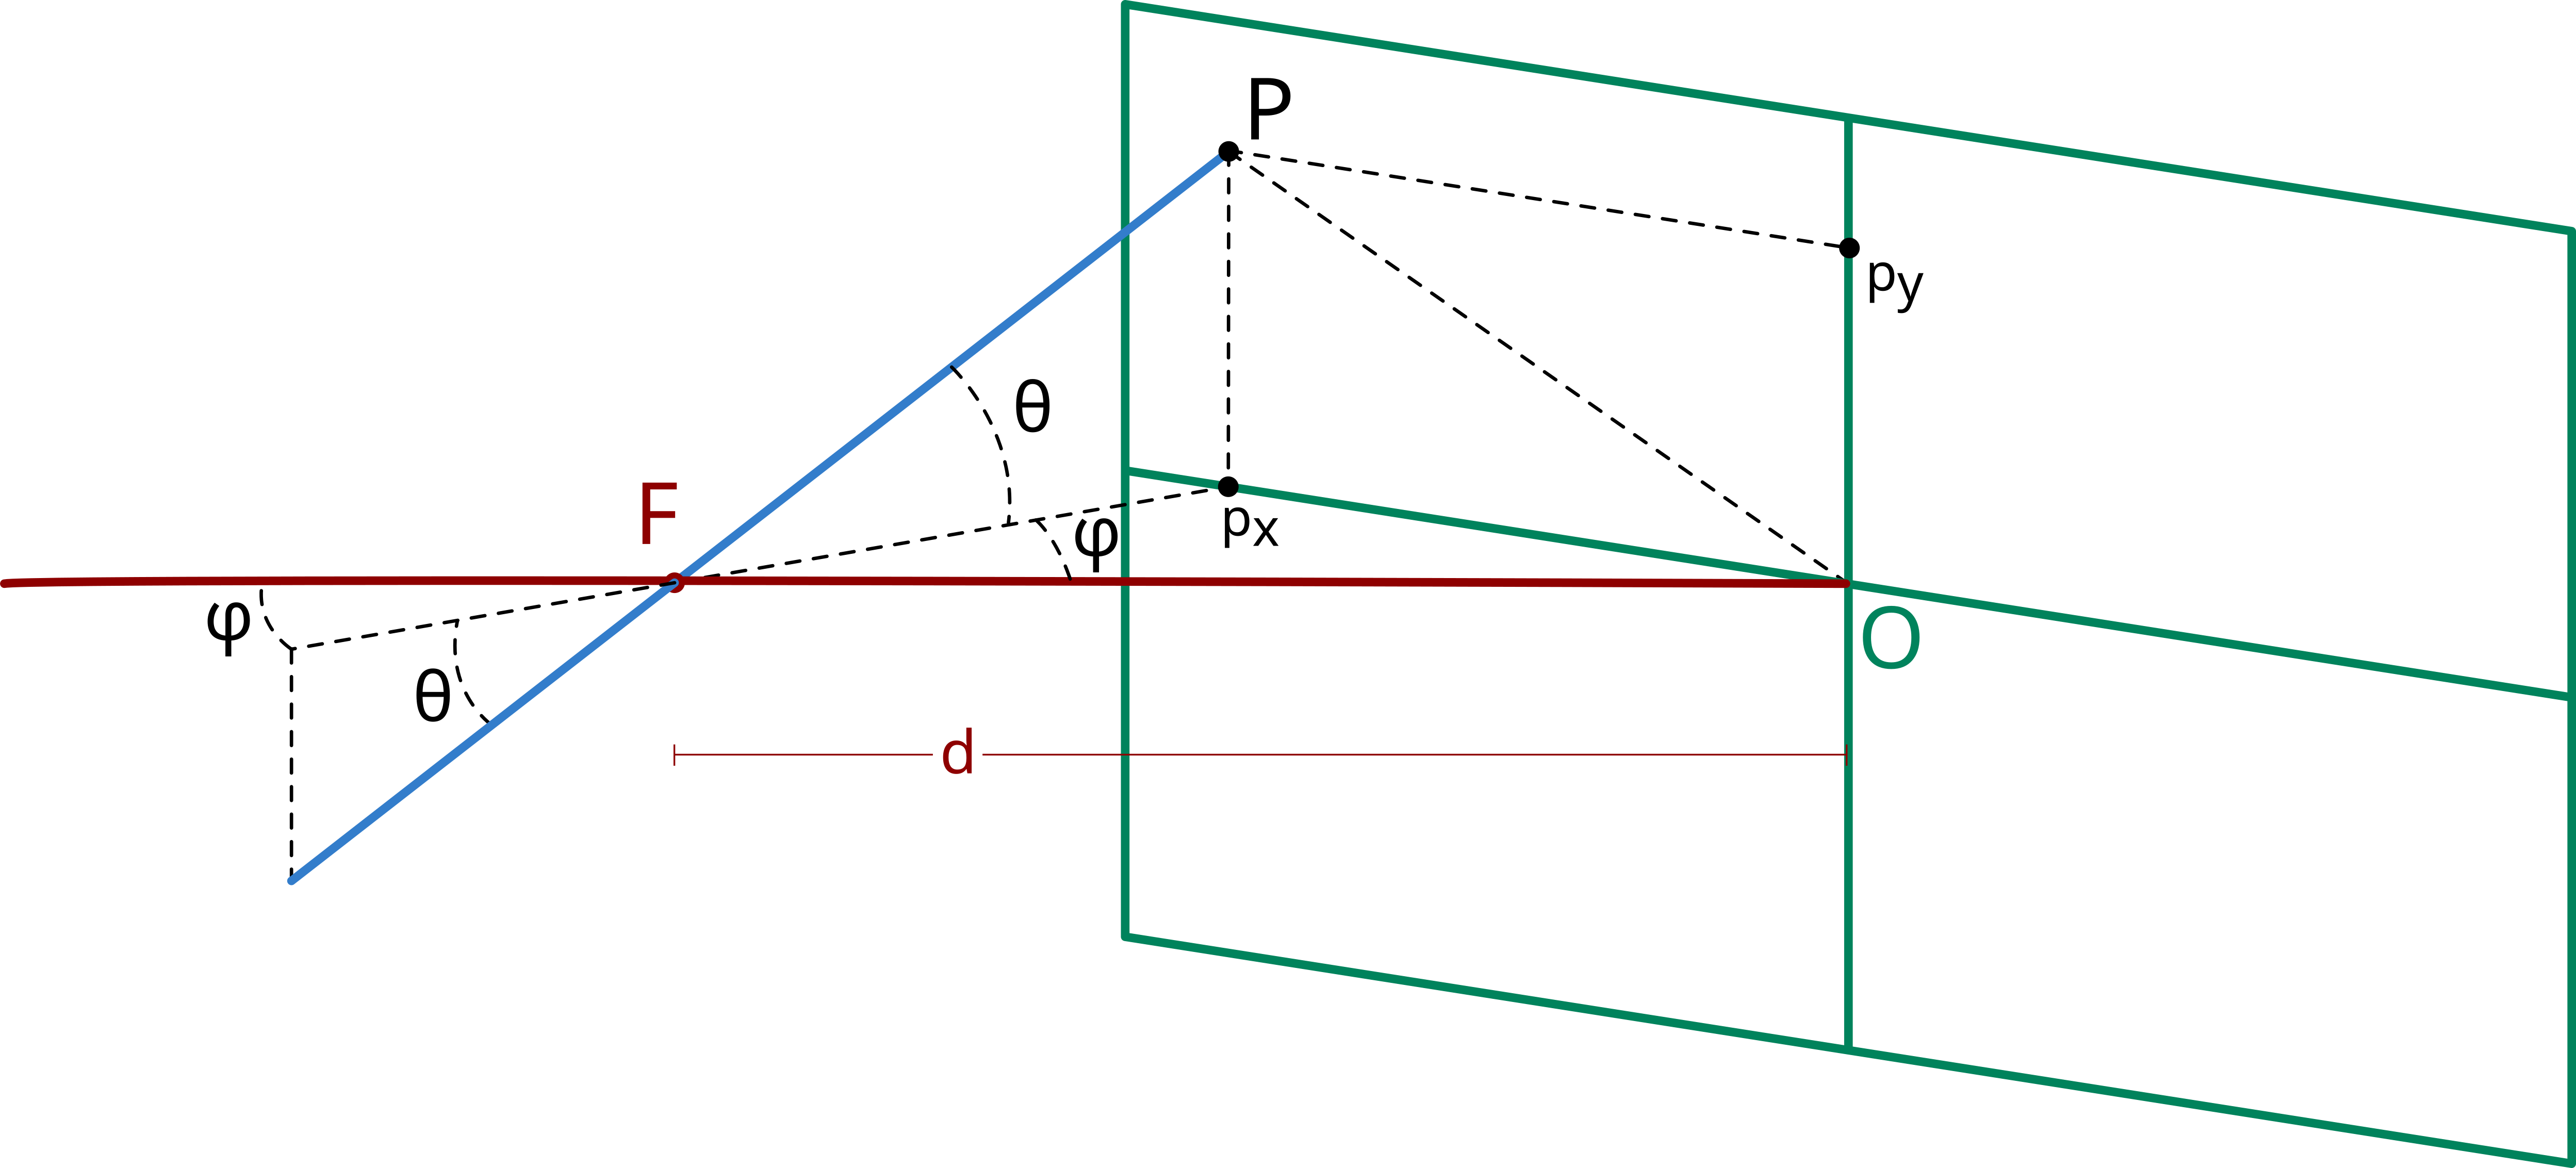
\includegraphics[width=.8\linewidth]{gfx/pinhole.png}
	\caption[Pinhole camera model]{Pinhole camera model}
	\label{fig:pinhole}
\end{figure}

All rays that hit the sensor are assumed, by our model, to pass through the focal point $F$. Thus, we can compute the angles $\vartheta$ and $\varphi$ for the ray hitting the sensor at pixel $P$ with elementary trigonometry.

From triangle $Fp_xO$ in \autoref{fig:pinhole}, we can obtain the angle $\varphi$ as
\[
	\varphi = \arctan{\frac{p_x}{d}}.
\]

Similary, the value of $\vartheta$ comes from the triangle $Fp_xP$ in \autoref{fig:pinhole}, which results in the following formula:
\[
	\vartheta = \arctan{\frac{p_y}{\sqrt{p_x^2 + d^2}}}.
\]

Finally, we need to adjust the zero for both $\vartheta$ and $\varphi$ to agree with the angle convention of the coordinate system. Therefore, the final formulas to computing the direction of an incoming ray hitting the camera's sensor ar a pixel $P = (p_x, p_y)$ are the following:
\begin{align}
	\vartheta_{cs} &= \frac{\pi}{2} + \arctan{\frac{p_y}{\sqrt{p_x^2 + d^2}}}, \\
	\varphi_{cs} &= \pi + \arctan{\frac{p_x}{d}}.
\end{align}

This discussion assumed the pixel coordinates to have its origin at the centre of the sensor. This is not the common coordinate system for pixels, as it usually have its origin at the top-left corner. A simple translation fixes that.

Finally, one should take into account the need to convert the pixel from the sensor coordinates to physical units. This is handled by computing the pixel width and height using the size of the sensor in physical units.

\subsection{Initial Conditions Computation}
\subsection{Ray Tracing}

\section{Parallelization Techniques}
\subsection{Classic Parallelization}
\subsection{General-Purpose Computing on Graphics Processing Units}